% !TEX TS-program = pdflatex
% !TEX encoding = UTF-8 Unicode

\documentclass[11pt,a4paper]{article}

\usepackage[utf8]{inputenc}

\usepackage[T1]{fontenc}
\usepackage[german]{babel}
\selectlanguage{german}

\usepackage{graphicx}
\usepackage{float}

\pagestyle{plain}

\title{SmartPi\\ \begin{large} Computer Architecture and Operating Systems\\ Universität Basel\end{large}}
\author{Eric da Costa, Alessandro Pittori}
\date{27. Januar 2019}

\begin{document}
\maketitle

\newpage

%\tableofcontents
\section{Inspiration}
Die Idee eines Webserver basierten Smart Homes kam uns erstmals, als die Beispielprojekte vorgestellt wurden. Unter diesen war eine Wetterstation, auf die man über einen Webserver zugreifen konnte. Wir hatten beide schon zuvor Erfahrung mit Webdesign und Alessandro zudem einen Überblick über das Webhosting, den Raspberry Pi und die Kombination der beiden. Er hat ein Smart Home Kit mit diversen Sensoren, das er bei einem Online Kurs des Hasso Platter Instituts gekauft hat. Weitere Inspiration kam von einem Smart Mirror Projekt des YouTube Kanals \textit{Hacker House}.

Es existieren viele Produkte auf dem Markt mit Smart Home Einbindung, das wohl bekannteste darunter ist die \textit{Philips Hue} Glühbirne. Auch alle Smart Speaker, wie das Amazon Echo, bieten Smart Home Funktionen wie das Verbinden einer solchen Glühbirne über das Drahtlose Netzwerk. Das Projekt soll uns einen Überblick über die Welt des Smart Homes geben und uns den Umgang damit aufzeigen.

\subsection{Umfang}
Das Produkt soll eine kompakte Kombination verschiedener Funktionalität sein. Es soll eine einfache Übersicht auf den Tag geben und den Haushalt unterstützen.
Dazu soll es einen Wecker beinhalten, der nach Ausschalten mittels Text-to-Speech über Lautsprecher den kommenden Tag beschreibt. Es soll ein Display besitzen, das neben Zeit und Wetter Kommende Kalenderevents und ungelesene E-Mail Nachrichten anzeigt. Zuletzt soll es die Temperatur und Luftfeuchtigkeit der Wohnung angeben und anzeigen, ob das Licht im Raum eingeschaltet ist. Als extra soll es eine Einkaufsliste zur Verfügung stellen, der man schnell und einfach Dinge hinzufügen kann, mit dem Gedanken, dass die Küche oft das Zentrum des Haushalts ist. Um das Produkt nicht an einen einzigen Raum zu binden, soll es alle Funktionalität über einen Webserver im Netzwerk zur Verfügung stellen, auf den man mit einem Computer oder Smartphone jederzeit zugreifen kann. Es soll so eine Zentrale Steuereinheit sein, die einfach erweitert werden kann.

Das Verbinden verschiedener Technologien steht hier im Zentrum. Das auslesen der Temperatur und Feuchtigkeitssensoren ist über Python sehr einfach. Die Programmiersprache, die wir am besten beherrschen ist Java. Ein Webbasiertes Interface geschieht über HTML oder ECMAScript (JavaScript). Wie können wir diese komplett unterschiedlichen Technologien miteinander verbinden? Wie kann dies \textbf{effizient} geschehen? Wie können alle Daten über verschiedene Webbrowser synchronisiert werden?

\section{Technologien}
Als Basis für das Projekt dient der Raspberry Pi. Als kleiner aber vollständiger Computer bietet er die Möglichkeit, jedes Programm auszuführen und besitzt zusätzlich eine einfache Stromschnittstelle für das auslesen der Sensoren. Er hostet einen Webserver, der alle Daten verwaltet. Dieser stellt die Rohdaten in einer API und eine Webapp als grafische Benutzeroberfläche zur Verfügung. Der Server und das Backend basieren auf Java. Das Web-Frontend ist eine React App, die die Daten über die SmartPi API mit \textit{fetch} abruft.

\subsection{APIs}
Die Abfrage nach neuen E-Mail geschieht über die Java Mail API. Wir haben diese generelle API gewählt um jegliche Adressen verwenden zu können und uns nicht auf einen Anbieter, wie z.B. Gmail, zu beschr\"anken. Im Gegensatz zur Verwaltung der E-Mails haben wir uns beim Kalender beschlossen \textit{Google Calendar} zu verwenden. Diese Wahl haben wir getroffen, weil wir es beide privat selbst  ben\"utzen und im Voraus wussten, dass es eine gut dokumentierte API dafür gibt. Für die Text-to-Speech Funktion haben wir uns für die Open Source Sprachsynthese Library MaryTTS entschieden. Es gibt viele kostenlose TTS Pakete, doch wir haben uns aufgrund der Vielfalt von Sprachen, Stimmen und Einstellungen für MaryTTS entschieden. Um die Wetterdaten abzurufen nutzen wir die API von OpenWeatherMap. Sie bietet kostenlos aktuelle Wetterdaten alle zehn Minuten und Fünftagesvorhersagen mit Datenpunkten alle drei Stunden.

\subsection{Hardware}
Die Hardware ist wegen der Budgetbeschränkung schlicht. Sie beinhaltet ein LCD Touchscreen für die Darstellung und Navigation der Webapp, einen Temperatur und Feuchtigkeitssensor und einen Lichtsensor. Für die Wiederhabe des Tons sind ein Set Stereolautsprecher verantwortlich. Das Gehäuse ist aus mit schwarzer Acrylfarbe bemaltem Holz. Das Herzstück ist ein Raspberry Pi 3B+.

\section{Aufteilung}
\subsection{Alessandro}
Alessandro hat das Design und die Implementierung der Webapp übernommen. Dazugehörig hat er sich um den Webserver und die API gekümmert. Die Wetterdaten werden direkt über die Webapp geladen. Ursprünglich war die Implementierung des Weckers in Java geplant und sollte von Eric übernommen werden, doch es hat sich im Laufe des Projekts herausgestellt, dass aus Effizienzgründen auch der Wecker direkt in der Webapp implementiert werden soll.

\subsection{Eric}
Eric hat bei dem Projekt die Java Programme für das Empfangen der E-Mails und der Kalenderdaten geschrieben. Die Interaktion mit den Sensoren, welche in Python programmiert wurde und die Kommunikation zwischen Python und Java wurden auch von ihm \"ubernommen. Zusätzlich hat er sich auch um die Text-to-Speech Funtkionalit\"at vom Projekt gek\"ummert. Die Daten werden dem Webserver über Methoden zur Verfügung gestellt.

\section{Implementierung}
\subsection{Architektur}
Als Webfrontend wird eine React App von einem Java HTTP Server gehostet. Die Pfadanfragen werden von verschiedenen Handlern verarbeitet. Es existiert ein Handler, der die React App und alle anderen benötigten Dateien serviert. Die restlichen Handler kommunizieren direkt mit den Klassen, die die E-Mails und die Kalenderdaten abrufen und die Sensordaten auslesen. Diese Daten werden im JSON Format als Antwort gesendet. So setzt sich die API zusammen, die E-Mails, den Kalender und die Sensordaten bereitstellt. Die Sensordaten werden von einem Python Script ausgelesen, das von einer Java Klasse ausgeführt wird. Der Server wird in eine ausführbare .jar-Datei verpackt.

\subsection{Wecker}
Alle Wecker sind als List in der React App verfügbar. Jede Sekunde wird überprüft, ob ein Wecker klingeln soll. Ist dies der Fall, wird eine Benutzeroberfläche angezeigt und ein Ton abgespielt. Die Benutzeroberfläche zeigt ein Weckersymbol, die Zeit und den Namen des Weckers und einen Knopf, der den Wecker abstellt.

\subsection{E-Mail}
Das Ziel bei der E-Mail war, dass man nur Nachrichten empfangen kann, da f\"ur das Projekt nicht geplant war auf E-Mails zu antworten. Um dies zu implementieren wurde, wie bereits erwähnt, die Java Mail API verwendet. Die E-Mail Adresse und das dazugehörige Passwort werden in einer Textdatei gespeichert und von Java geparsed. Es existiert eine Klasse, worin die Nachrichten geladen und gespeichert werden. Der Server greift anschliessend auf diese Klasse zu und bekommt die E-Mails als Liste von Maps. Diese Liste beinhaltet den Sender, den Betreff und die Nachricht selber.

\subsection{Kalender}
Mit Hilfe der ausführlichen Dokumentation von Google ist die Implementierung vom Kalender ohne Probleme geschehen. In einer Kalender Klasse mit einer Methode um die zukünftigen Termine zu laden und speichern. Der Server kann dann im gleichen Stil wie bei den E-Mails auf diese Methode aufrufen und bekommt eine Liste von Maps mit den Namen und den Zeiten. Um auf den Kalender zugreifen zu können, muss eine JSON-Datei von Google heruntergeladen werden mit den nötigen Anmeldedaten.

\subsection{Sensoren}
Die verwendeten Sensoren wurden mit einem Python Skript ausgelesen und entsprechend ausgewertet. Die Daten werden bei jedem Aufruf des Skripts \textit{geprintet}. Die Python Skript wird in einer Java Klasse ausgeführt und die geprinteten Daten dort geparsed. Der Server ruft indirekt das Python Skript auf und bekommt die Daten, um diese dann weiterzuverwenden.

\subsection{Text-to-Speech}
Nach dem der Wecker vom Benutzer ausgeschaltet wurde, wird von der Text-to-Speech Funktionalit\"at zuerst das n\"achste Event vorgelesen und anschliessend alle neuen Nachrichten. MaryTTS bietet eine grosse Auswahl an Effekte und Stimmen, jedoch haben wir beschlossen es bei der normalen Stimme zu lassen. Falls keine neuen Ereignisse oder Nachrichten existieren, wird dies natürlich so wiedergegeben.

\subsection{Webserver}
Der Webserver ist ein \textit{HttpServer} der \textit{org.sun.net} Library. Dieser hört auf Port 80 anfragen ab. Für die verschiedenen Anfragepfade existieren Handler, die mit Pfaden verknüpft werden und so zu einem Kontext werden. Wenn ein Pfad von einem Webbrowser angefragt wird, wird der Handler ausgeführt. Es existiert ein Handler, der die React App und alle benötigten Dateien serviert. Der Rest der Handler ist für die API zuständig.

\subsection{React}
Die React App ist aus mehreren Seiten zusammengesetzt. Es existiert eine Homepage, auf der eine Zusammenfassung dargestellt ist. Auf ihr findet man eine Uhr, das Datum und den kommenden Wecker mit einem Knopf um Wecker hinzuzufügen. Das aktuelle Wetter, die Wohnungstemperatur und Feuchtigkeit sowie der Status des Lichts sind daneben abgebildet. Anschliessend findet man eine Einkaufliste komplett mit Knopf zum hinzufügen von Produkten. Im unteren Teil finden sich die heutigen Kalenderevents und daneben die E-Mails. Weitere Seiten, die Details zu allen Kalender Events, E-Mails, Weckern und der Wettervorhersage sind über Links zugänglich. Diese zeigen jeweils alle Events des Kalenders, alle E-Mails und deren Inhalt und die fünf Tage Vorhersage des Wetters.
\begin{figure}[H]
\includegraphics[width=1\textwidth]{images/home.png}
\includegraphics[width=.5\textwidth]{images/alarms.png}
\includegraphics[width=.5\textwidth]{images/forecast.png}
\includegraphics[width=.5\textwidth]{images/calendar.png}
\includegraphics[width=.5\textwidth]{images/email.png}
\caption{Screenshots mit arbiträren Daten}
\end{figure}

\subsection{Gehäuse und Zusammenbau}
Das Gehäuse besteht aus zugeschnittenem Sperrholz. Es ist sowohl aussen als auch innen mit schwarzer Acrylfarbe bemalt. Die Front hat einen Ausschnitt für das Display, wodurch es Flach mit der Aussenseite liegt. Zwei Löcher für die Lautsprecher sind an der Unterseite ausgeschnitten. Die Lautsprecher sind, ohne bessere Methode, mit starkem Klebeband festgeklebt. Oben ist ein kleines Loch für den Lichtsensor. Der Raspberry Pi ist auf einer Brücke über der Rückseite des Displays montiert. Die ganze Vorderseite ist mit den Seitenwänden fest verschraubt und kann bei belieben für Wartungszwecke entfernt werden. Das Sensorarray ist an einem Stück Holz, das auf die Grundplatte geklebt ist, montiert. Die Sensoren sind über ein selbstgelötetes Verlängerungskabel verbunden.

\begin{figure}[H]
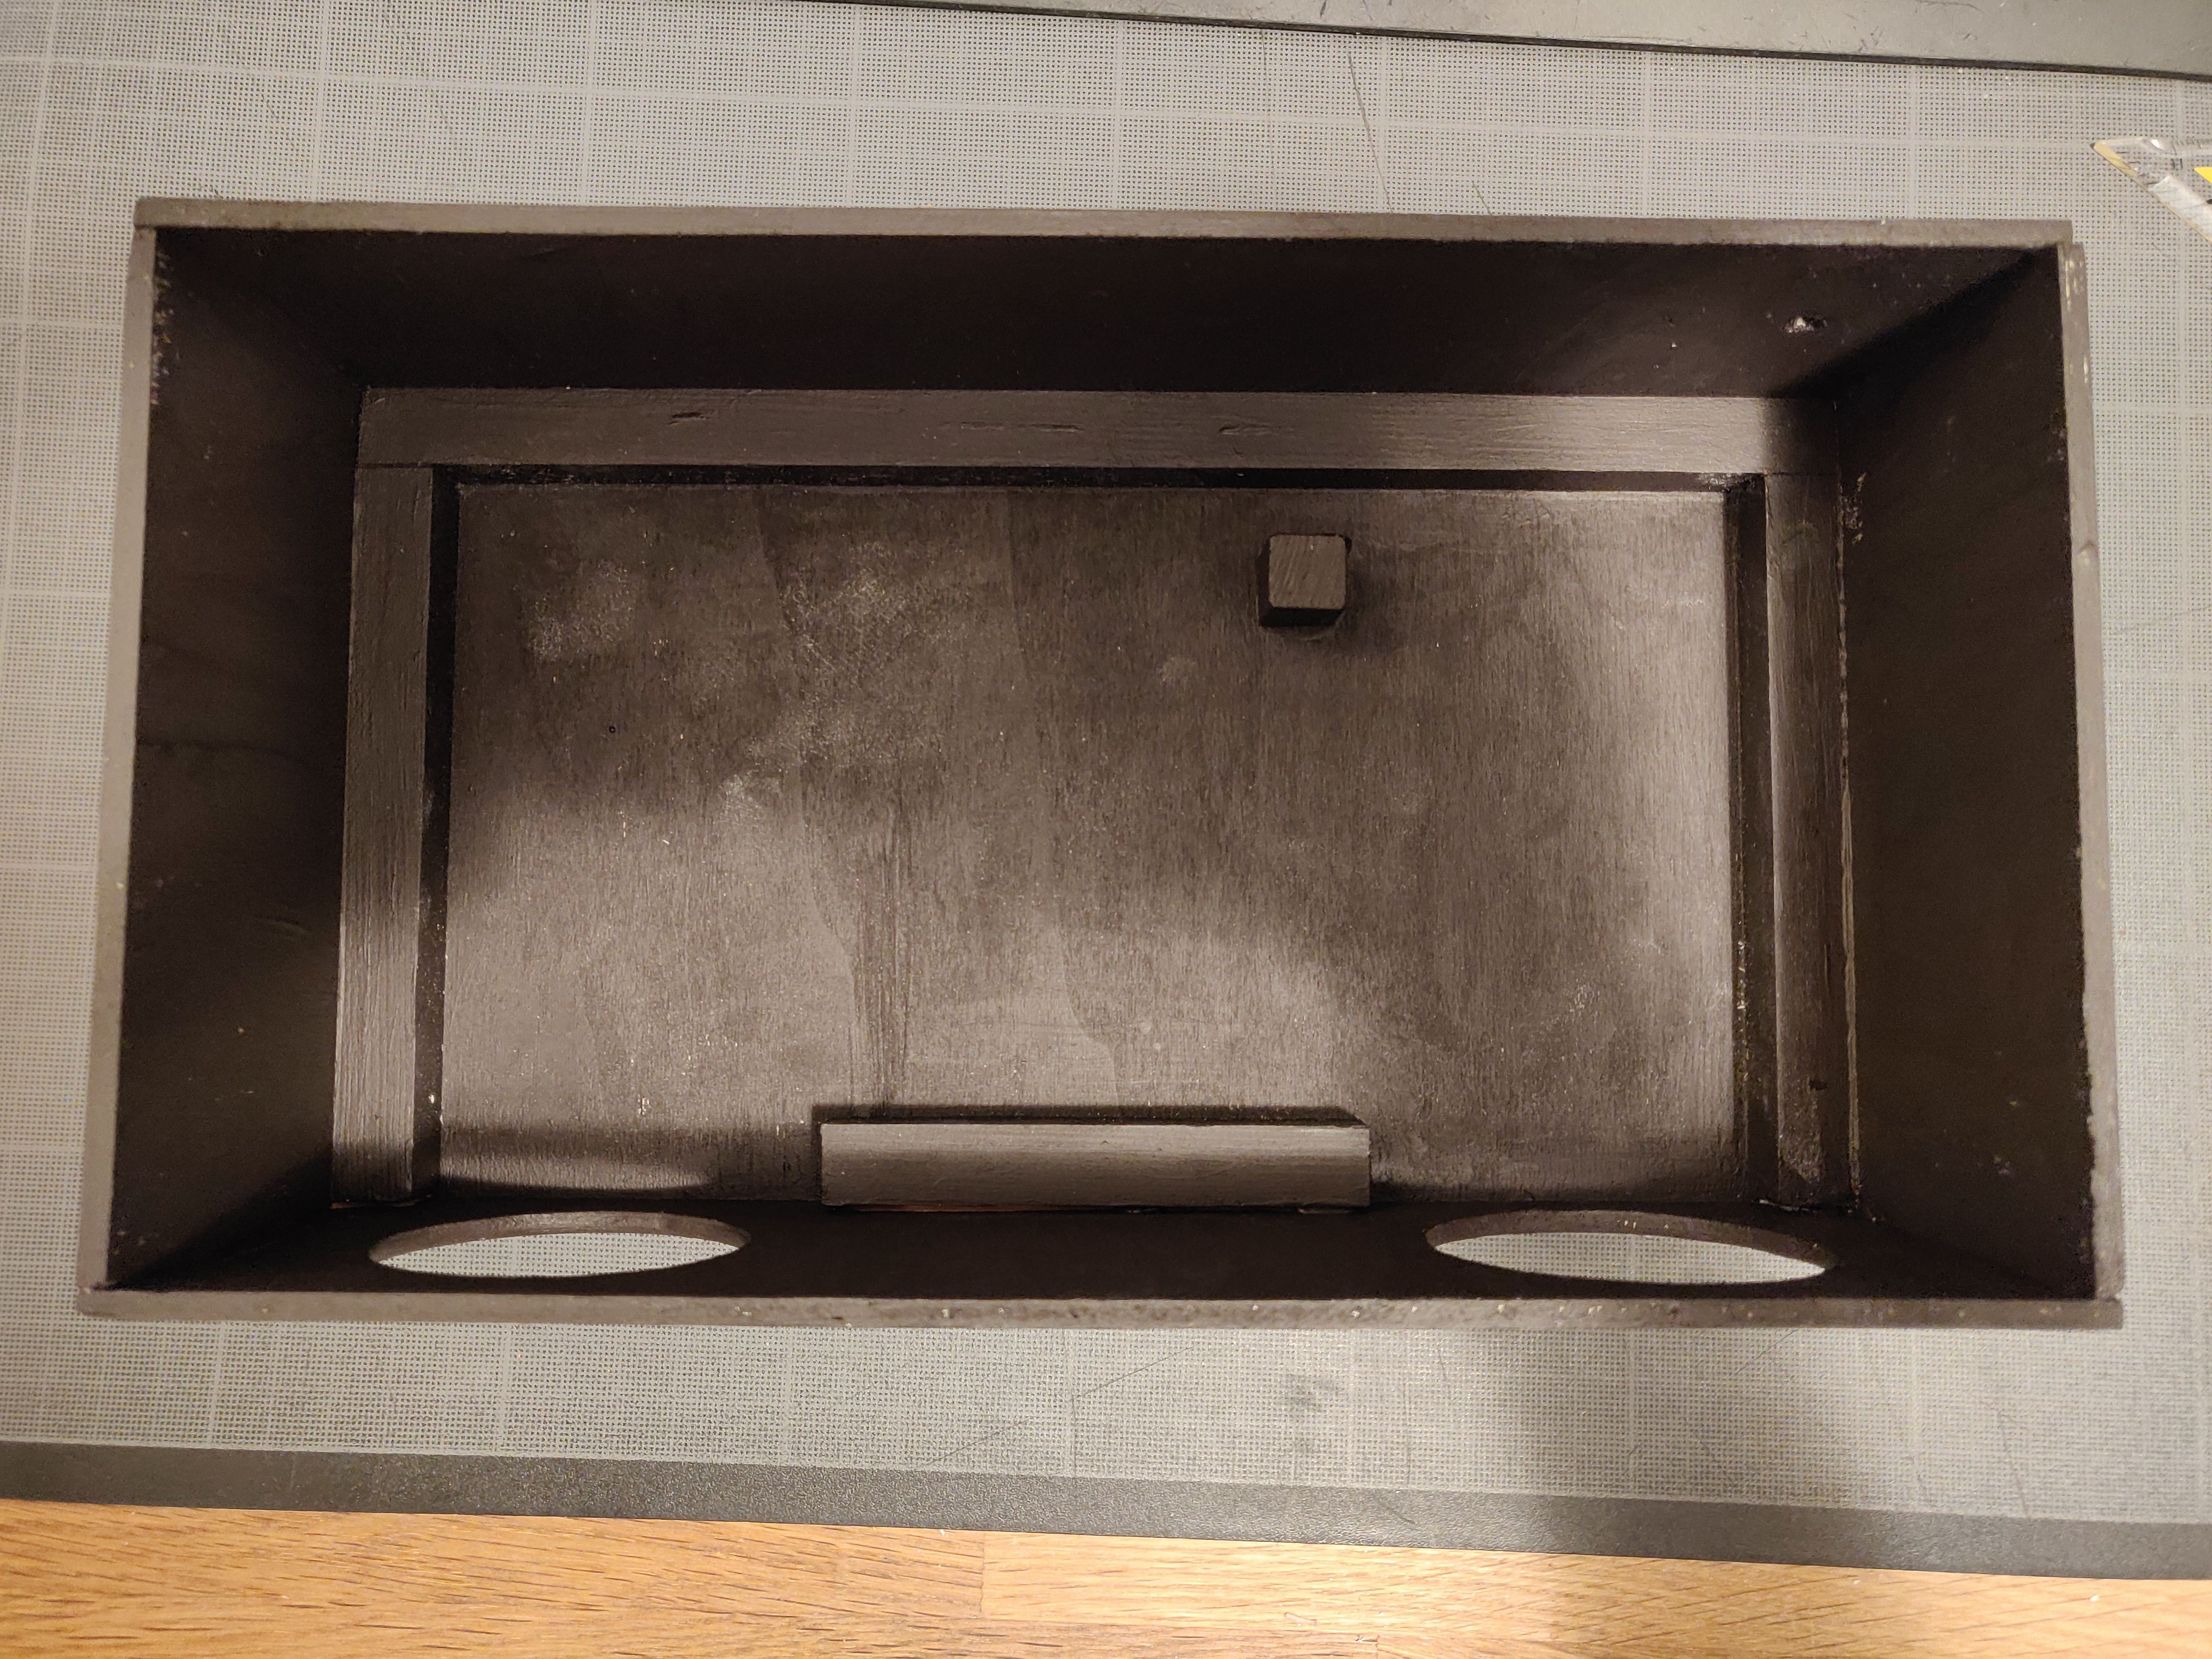
\includegraphics[width=.5\textwidth]{images/hard1.jpg}
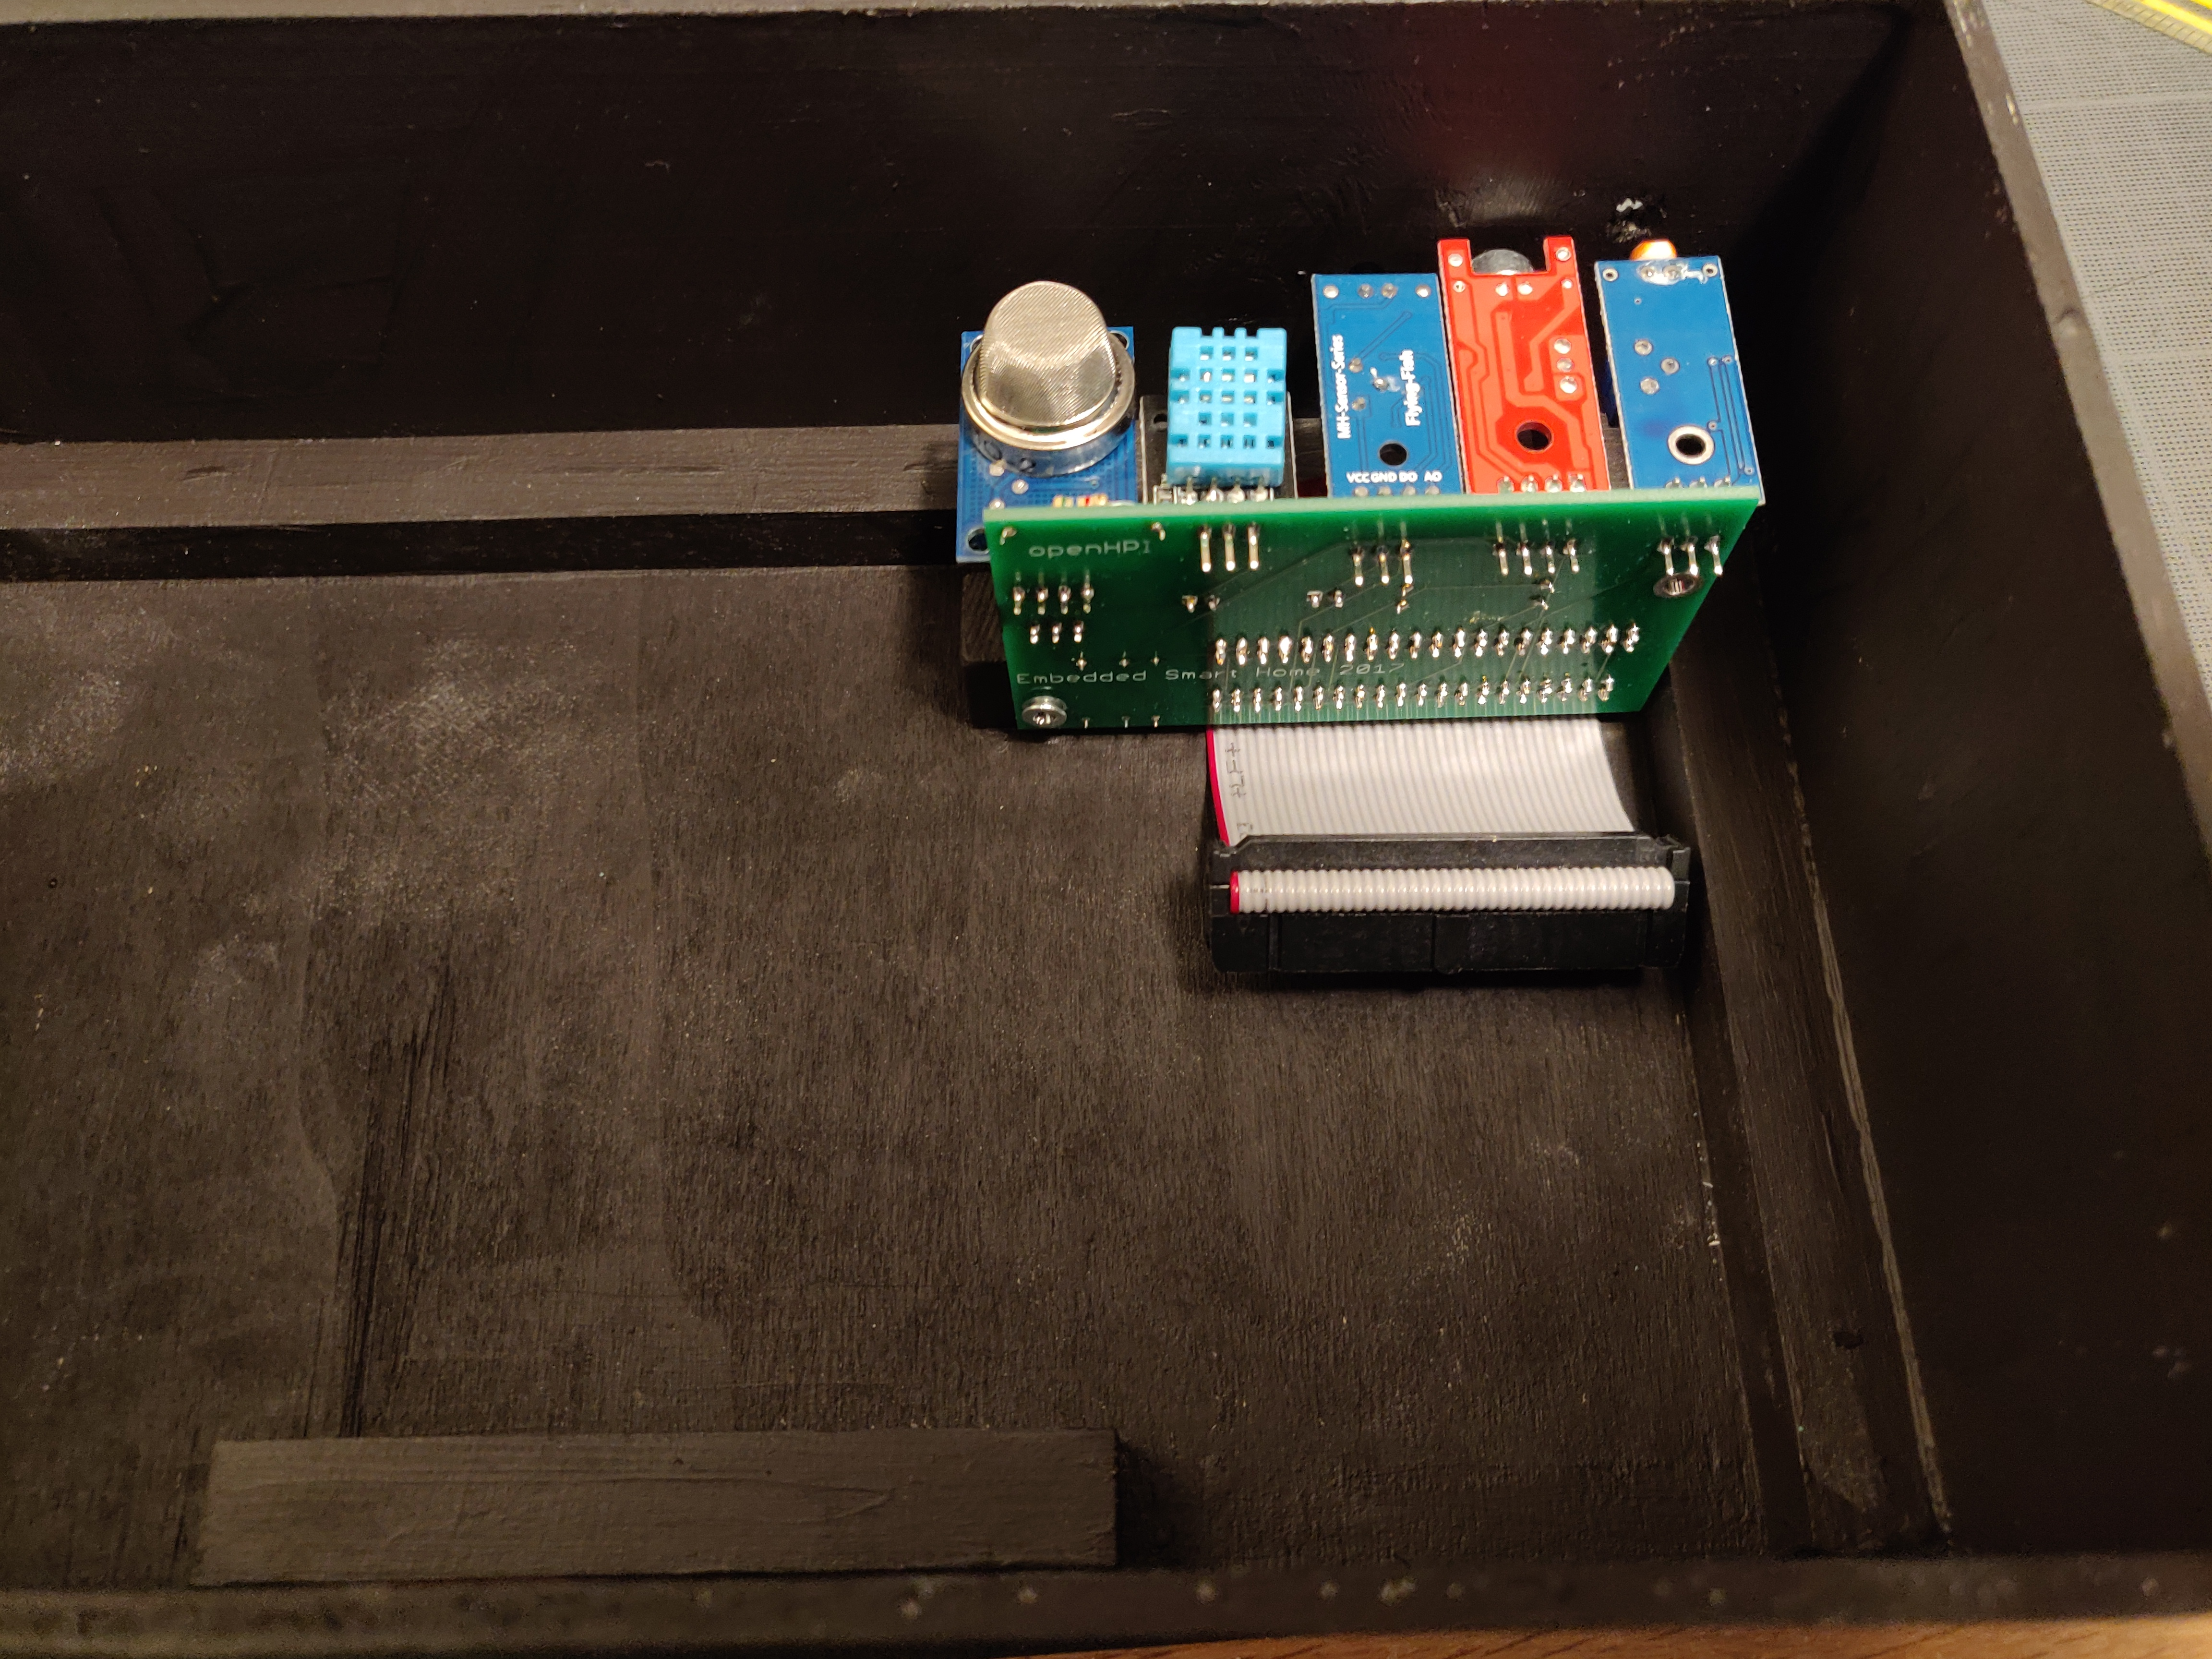
\includegraphics[width=.5\textwidth]{images/hard2.jpg}
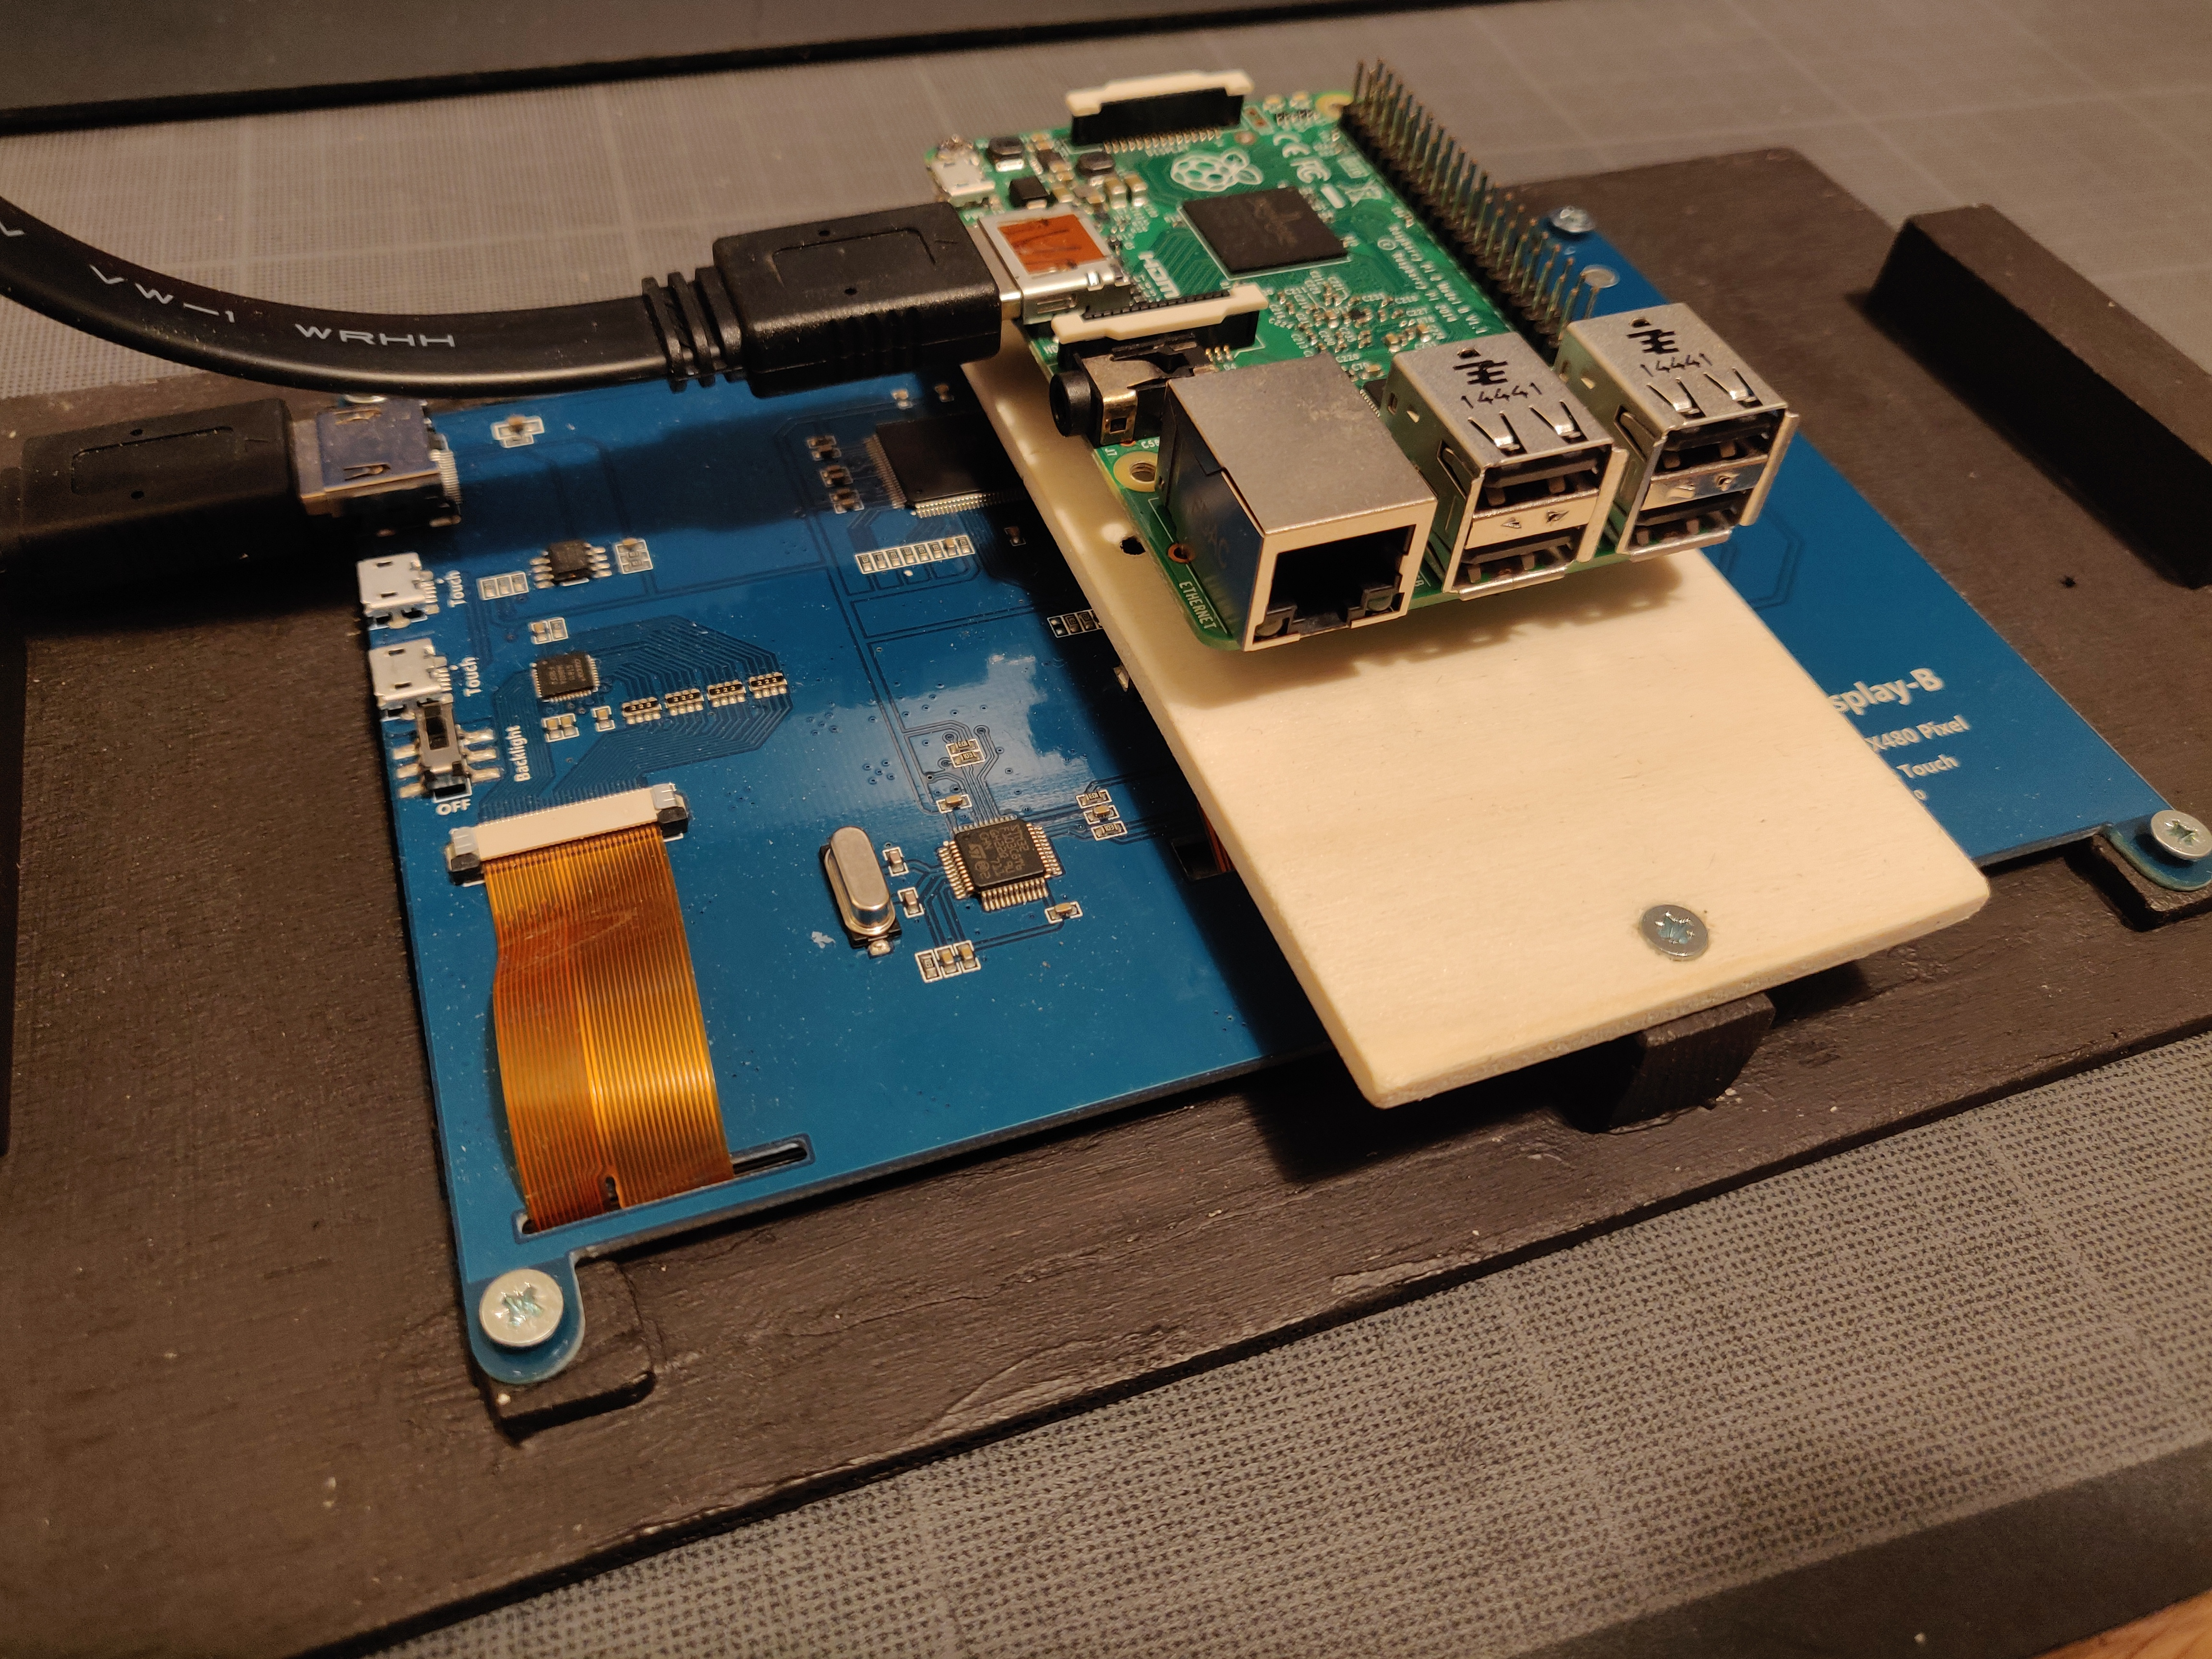
\includegraphics[width=.5\textwidth]{images/hard3.jpg}
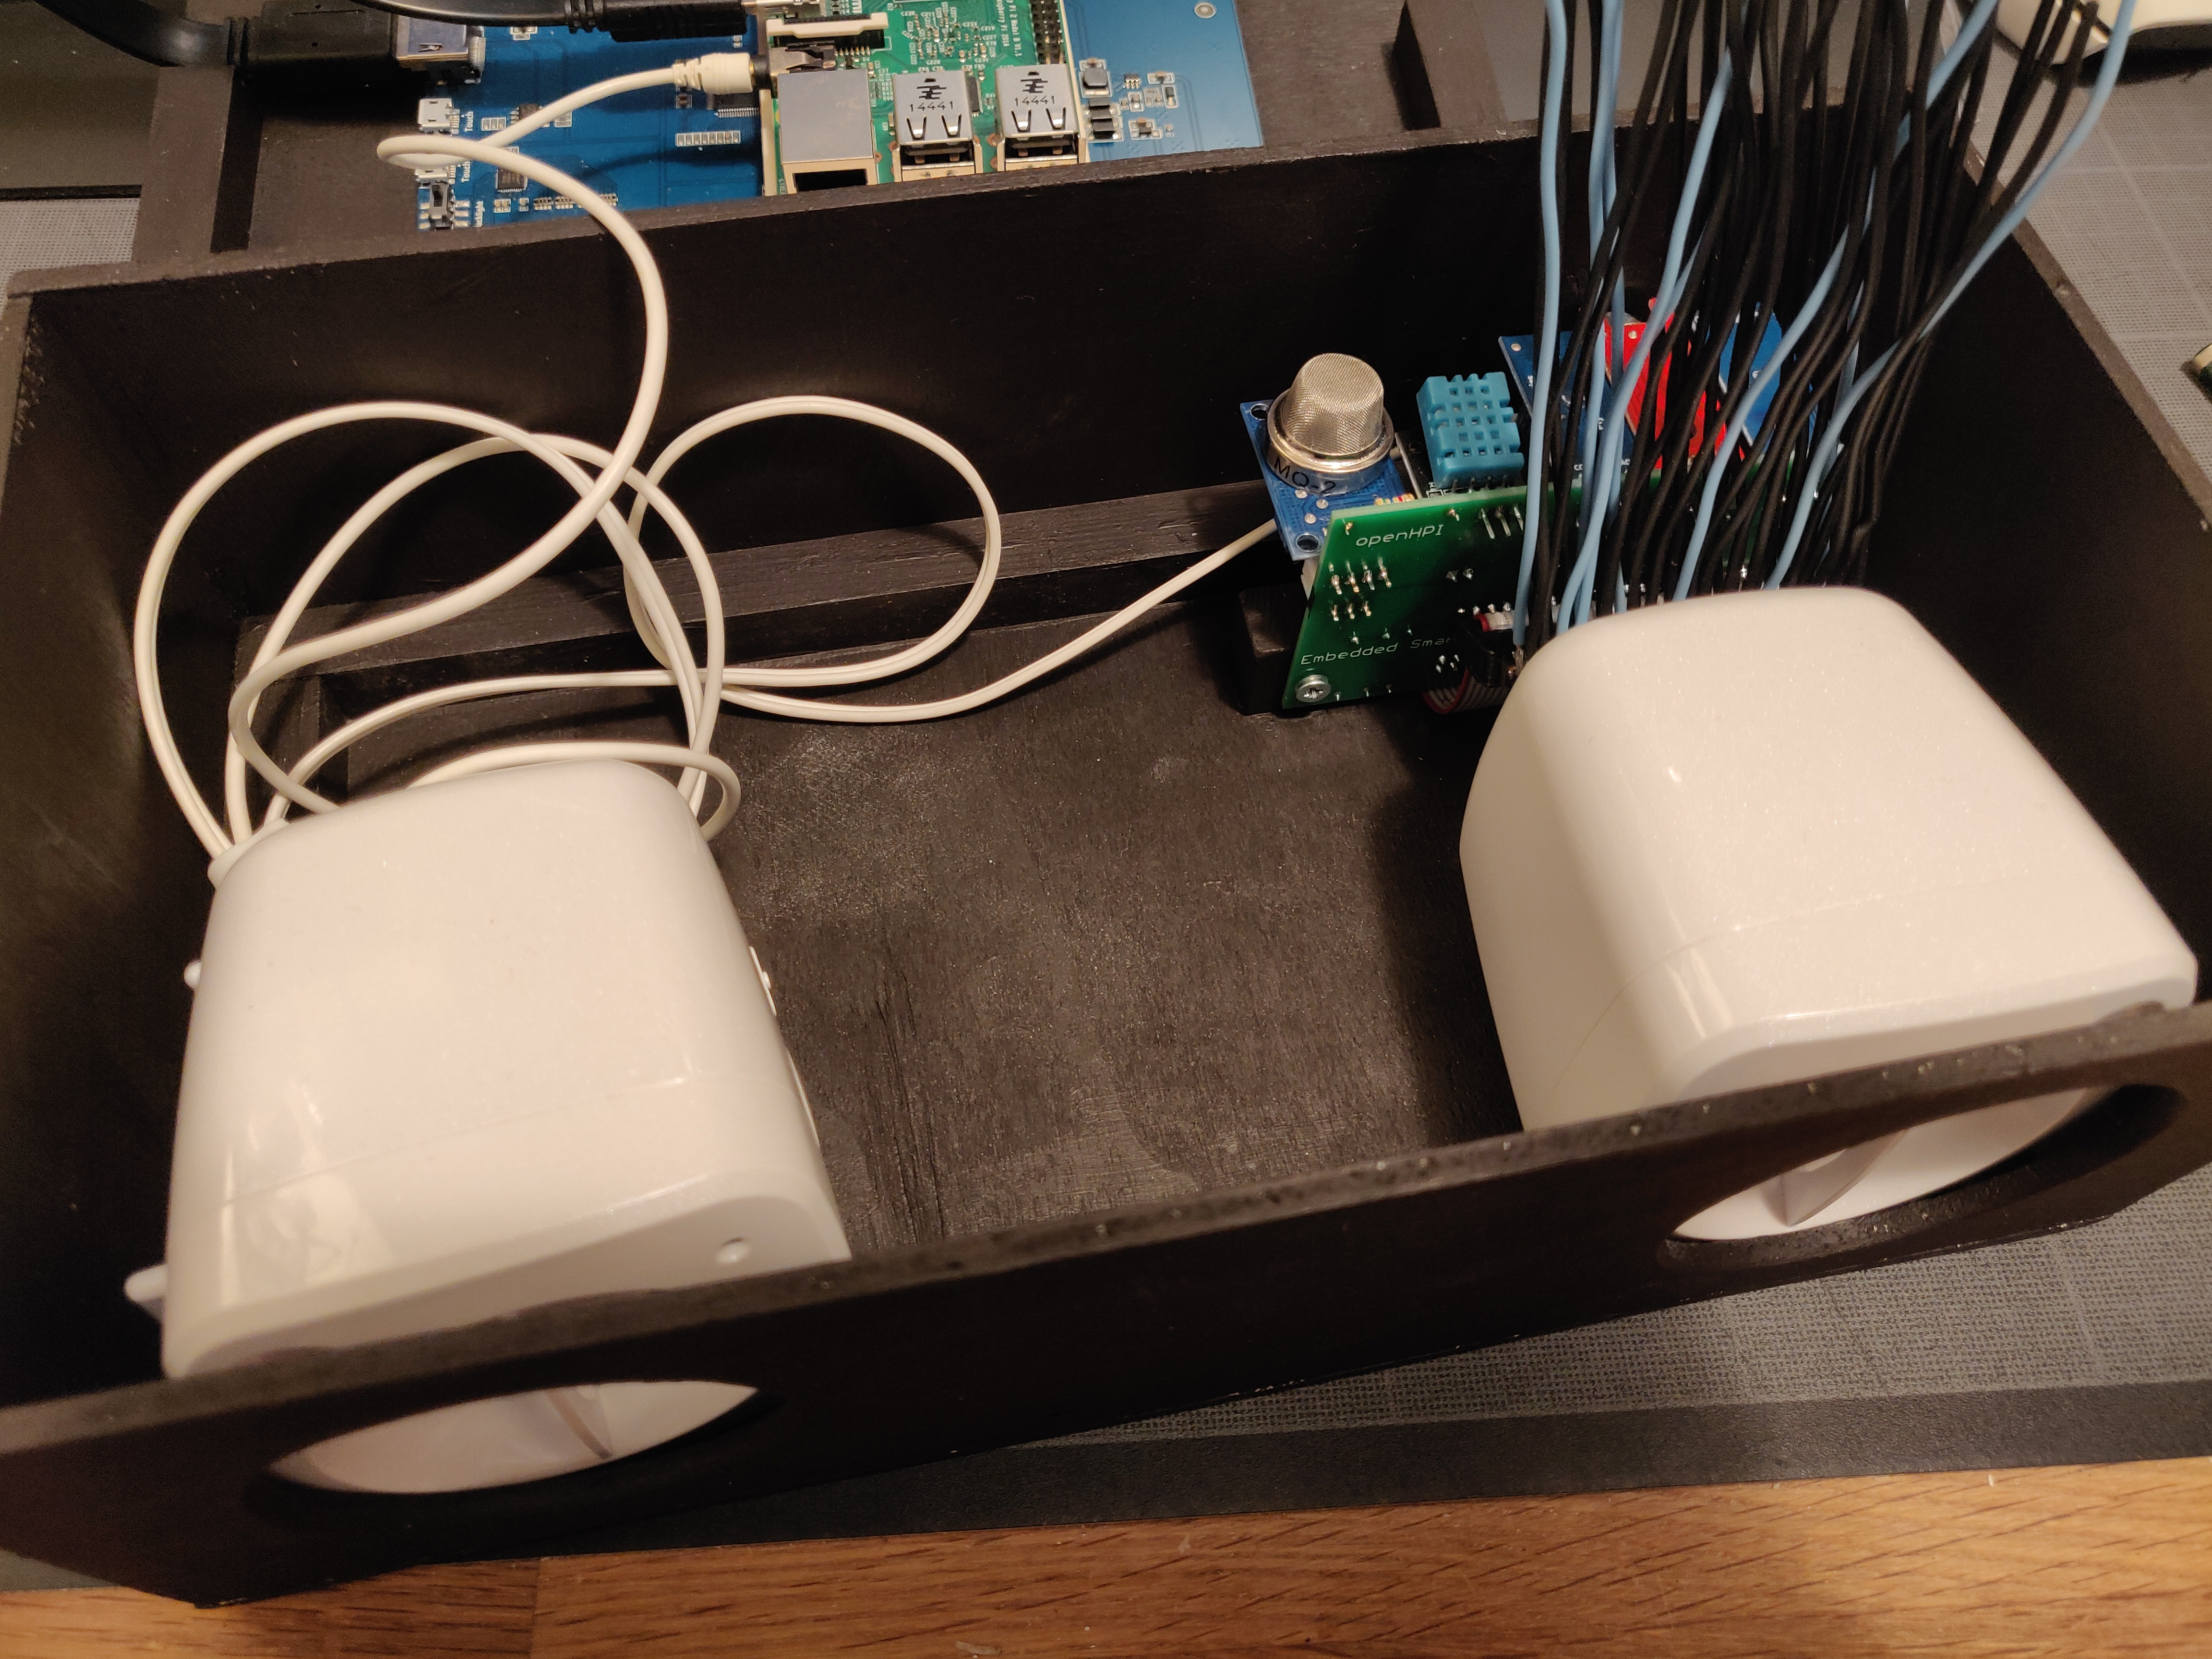
\includegraphics[width=.5\textwidth]{images/hard4.jpg}
\includegraphics[width=.5\textwidth]{images/hard5.jpg}
\end{figure}

\section{Abschliessend}
\subsection{Resultat}
Wir haben das Erreicht, was wir uns vorgenommen haben. Neben unseren Mindestanforderungen, einem Display, Webserver und Webapp, dem Wecker, des Temperatursensors und der Wettervorhersage, haben wir Text-to-Speech, Feuchtigkeits und Lichtsensor und eine ansprechende Benutzeroberfläche auf die man von jedem Webbrowser im Netzwerk zugreifen kann.

\subsection{Fazit}
Wir sind von der Inspiration der Wetterstation im Lauf des Projekts auf den Fokus der Kommunikation der verschiedenen Technologien gekommen. Wir haben viel Erfahrung mit dem Verbinden der Technologien gesammelt, u.A. den Webserver direkt in Java zu implementieren. In der Vorlesung Software Engineering haben wir parallel zu diesem Projekt ein streng strukturiertes Verfahren kennengelernt, was auf dieses Projekt abgefärbt hat. Trotzdem hätten wir uns zeitlich besser strukturieren und unsere Ideen besser planen und durchdenken können.
Wir sind mit dem Resultat sehr zufrieden und haben vor, es weiter auszubauen. Eines unserer Designziele war Anpassbarkeit und Erweiterbarkeit, welches wir sehr gut erreicht haben.

\section{Literatur}
https://developers.google.com/calendar/quickstart/java \newline
https://javaee.github.io/javamail/ \newline
http://mary.dfki.de \newline
https://www.youtube.com/channel/UCj7qnP36Ye7gsiqvhA3eALw \newline
https://www.youtube.com/watch?v=fkVBAcvbrjU \newline
https://open.hpi.de/ \newline
https://openweathermap.org/api
%\bibliographystyle{plain}
%\bibliography{CAOS-Project-Report_SmartPi_Eric_da_Costa_Alessandro_Pittori}

\end{document}
